\documentclass{article}
\PassOptionsToPackage{numbers,compress}{natbib}
\usepackage[final]{neurips}
\usepackage[utf8]{inputenc}
\usepackage[T1]{fontenc}
\usepackage{booktabs}
\usepackage{amsmath,amsfonts,amssymb}
\usepackage{graphicx}
\usepackage{microtype}
\usepackage{xcolor}
\usepackage{array}
\usepackage{float}
\usepackage{enumitem}
\usepackage[hidelinks]{hyperref}
\setlist{nosep,leftmargin=*}
\setlength{\textfloatsep}{4pt plus 1pt minus 1pt}
\setlength{\floatsep}{3pt plus 1pt minus 1pt}
\setlength{\intextsep}{3pt plus 1pt minus 1pt}
\newcommand{\R}{\mathbb{R}}

\title{Learning Spatial Unit-Norm Latents with Riemannian Flow Matching}
\author{Mohammadreza Tavasoli Naeini \\
Department of Electrical and Computer Engineering, University of Toronto \\
\texttt{mohammadreza.tavasolinaeini@mail.utoronto.ca}}

\begin{document}
\maketitle

\begin{abstract}
Latent generative models often use a Gaussian prior, but an autoencoder is not forced to produce Gaussian latents. Its architecture and normalization can instead create features with nearly constant norm; normalized Transformer encoders are one example. We study a simple design rule: the prior should match the latent support learned by the autoencoder. We introduce Spherical Riemannian Unit-Norm Latents (SRUL), which trains an autoencoder to produce spatial unit-norm tokens and learns their distribution with Riemannian Flow Matching (RFM) on the same product-of-spheres support. On CIFAR-10, replacing a straight chord with geodesic transport improves FID from $67.44$ to $63.84$ when the spherical autoencoder is unchanged. In a support-matching comparison, SRUL reaches FID $49.42$, compared with $50.70$ for VAE + standard FM and $56.04$ when the same VAE latents are projected to directions before RFM. Tangent-noise and classifier-free-guidance ablations study the main controls, while PathMNIST and CelebA-64 test the method in additional image settings.
\end{abstract}

\section*{Attestation of Teamwork}
Mohammadreza Tavasoli Naeini conducted the background study, designed and implemented the models, ran and analyzed the experiments, and prepared the report, presentation, and code.

\section{Introduction}
Latent generative models have two parts. An autoencoder first maps an image to a latent code, and a prior then learns how to generate new codes for the decoder. Gaussian latents are common, especially in VAE-based models, but the encoder is free to learn a different geometry. Normalization can make token norms nearly constant, so information is carried mainly by direction. Transformer encoders with LayerNorm are one example, and explicit $L_2$ normalization can create the same structure in a convolutional encoder.

The prior should therefore be chosen after considering the latent support. When an encoder produces spherical tokens, standard linear interpolation is not well matched to them: even if both endpoints have unit norm, the straight path is a chord through the sphere's interior. The reverse mismatch can also occur. A VAE may use both token direction and token magnitude; projecting its latents onto a sphere after training removes the magnitude information that its decoder expects.

To study this support-matching principle, we introduce Spherical Riemannian Unit-Norm Latents (SRUL). Its autoencoder learns a spatial grid of unit-norm tokens, and its RFM prior learns a probability path on the same product of spheres. The representation and prior are therefore trained for the same latent support instead of being connected by a post-hoc projection.

We study the design with two controlled tests. First, we keep the spherical autoencoder unchanged and compare a Euclidean chord with geodesic RFM transport. Second, we compare SRUL with a VAE modeled by standard FM and with the same VAE after its latents are reduced to directions for projected RFM. The second test shows whether a spherical prior can be attached to a VAE after training without losing radial information. We also study the tangent-noise scale and classifier-free guidance, then evaluate the same SRUL pipeline on CIFAR-10, PathMNIST, and CelebA-64.

\section{Related Work and Positioning}
Variational autoencoders learn stochastic Euclidean latents and use a KL term to regularize them toward a Gaussian prior \cite{vae}. Latent Diffusion Models then move generation from pixels to such a learned latent grid, reducing computation while preserving perceptually important information \cite{ldm}. Unified Latents studies how encoder noise controls the information passed through a latent representation, while keeping a Euclidean generative process \cite{ul}. Sphere Encoder explicitly maps images to a sphere and trains the decoder to remain stable around encoded points, with the goal of direct sampling from an approximately uniform spherical distribution \cite{sphere}.

Flow Matching learns a time-dependent velocity field along a chosen probability path \cite{fm}. Standard linear Flow Matching uses straight paths in Euclidean latent space. RJF observes that normalized representation encoders often produce features with nearly constant norm and replaces this interpolation with Riemannian Flow Matching on the sphere; it also studies an additional Jacobi weighting \cite{rjf}. SRUL differs in two ways. It learns the spatial spherical representation rather than assuming a pretrained representation encoder, and it uses tangent perturbation as a controllable latent bottleneck. This makes encoder--prior co-design, rather than only applying RFM to an existing representation, the central question. The final method uses the RFM formulation because it was the strongest variant in our experiments.

\section{Method}
\subsection{Pipeline overview}
Figure~\ref{fig:pipeline} shows the full pipeline. Representation learning produces a grid of unit-norm tokens and trains the decoder to remain stable under tangent perturbations. RFM then learns the distribution of these encoded tokens using geodesic paths and tangent velocities. During sampling, spherical noise is transported with exponential-map steps and decoded into a new image.

\begin{figure}[H]
\centering
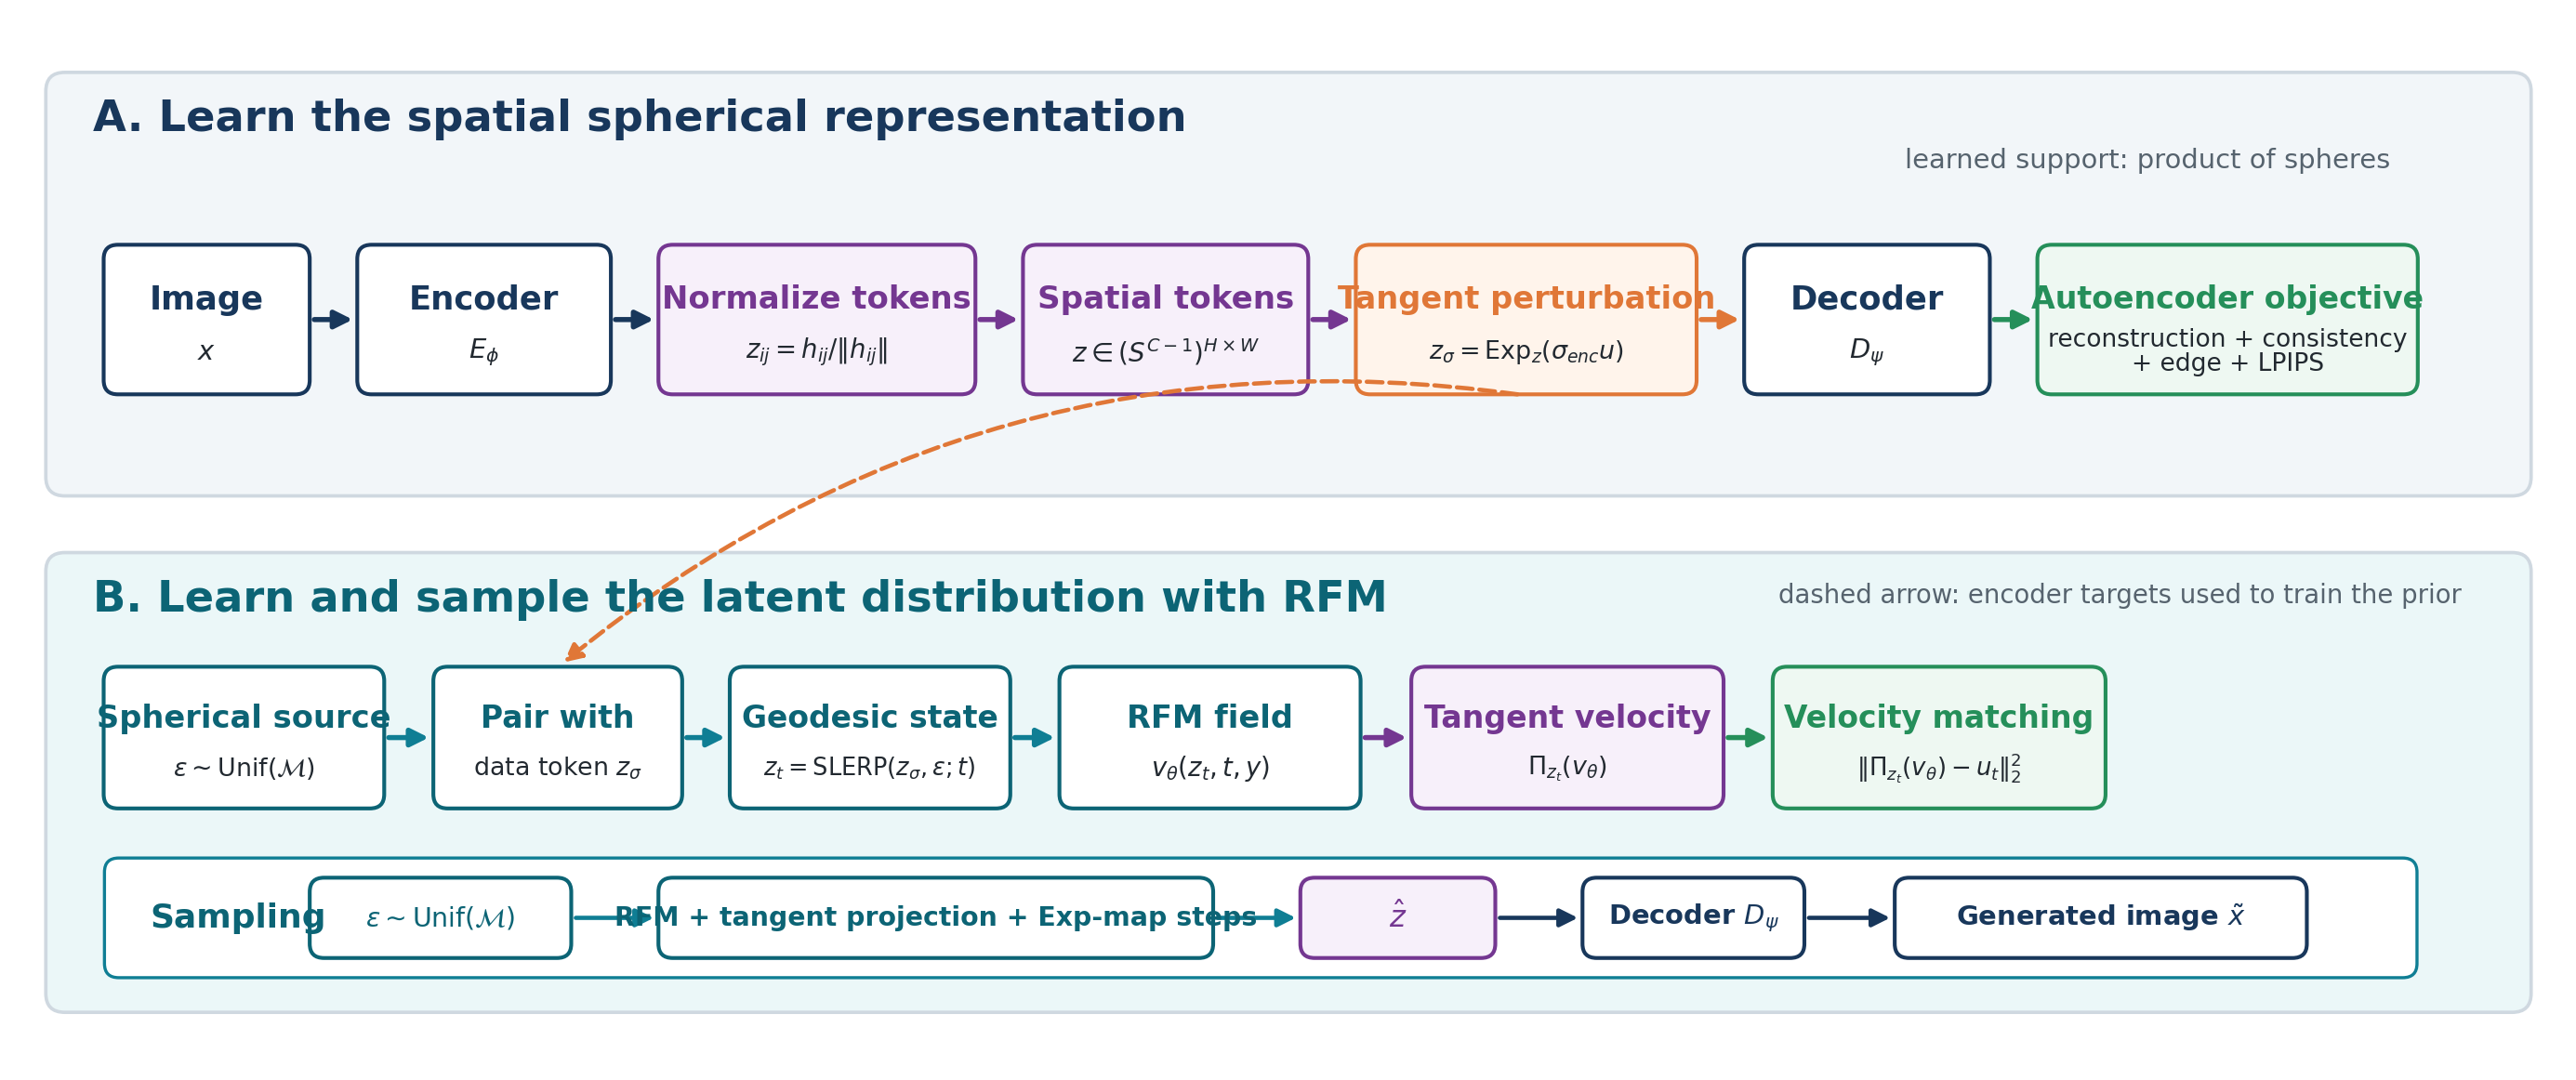
\includegraphics[width=0.95\linewidth]{assets/srul_pipeline_v10.png}
\caption{SRUL pipeline. The first stage learns spatial spherical tokens and a decoder robust to tangent perturbations. The second stage learns and samples an RFM prior on the same product-of-spheres manifold. Class labels and classifier-free guidance are optional conditional inputs.}
\label{fig:pipeline}
\end{figure}

\subsection{Spatial spherical autoencoder}
For an image $x$, the encoder produces a spatial tensor
\begin{equation}
 h=E_\phi(x)\in\R^{C\times H\times W},\qquad
 z_{:,i,j}=\frac{h_{:,i,j}}{\|h_{:,i,j}\|_2}\in S^{C-1}.
\label{eq:encoder}
\end{equation}
The full latent space is $\mathcal M=(S^{C-1})^{HW}$. We use $C=32$, a $4\times4$ token grid for $32\times32$ images, and an $8\times8$ grid for CelebA-64. The constraint is imposed during representation learning; it is not added after an unconstrained autoencoder has already decided how to use token magnitude.

The autoencoder is trained from clean and perturbed latents:
\begin{align}
\mathcal L_{\mathrm{AE}}={}&
\lambda_c\|D_\psi(z)-x\|_1
+\lambda_n\|D_\psi(z_\sigma)-x\|_1
+\lambda_e\mathcal L_{\mathrm{edge}} \nonumber\\
&+\lambda_{\mathrm{lat}}\big[1-\cos\big(z,E_\phi(D_\psi(z_\sigma))\big)\big]
+\lambda_p\mathcal L_{\mathrm{LPIPS}}.
\label{eq:ae}
\end{align}
The clean and noisy reconstruction terms preserve image content, while latent consistency, edge loss, and LPIPS improve local stability and perceptual detail.

\subsection{Tangent-noise control}
For each token, Gaussian noise is projected onto the tangent space,
\begin{equation}
 \xi\sim\mathcal N(0,I),\qquad
 u=\Pi_z(\xi)=\xi-\langle\xi,z\rangle z,
\end{equation}
and the perturbed token is
\begin{equation}
 z_\sigma=\operatorname{Exp}_z(\sigma_{\mathrm{enc}}u).
\label{eq:noise}
\end{equation}
Because $u\perp z$, this operation changes direction without changing radius. The scalar $\sigma_{\mathrm{enc}}$ controls angular perturbation and retained image information.

\subsection{Riemannian Flow Matching prior}
The source is uniform on the same manifold, $\epsilon\sim\operatorname{Unif}(\mathcal M)$. For a data latent $z_\sigma$ and source sample $\epsilon$, the tokenwise geodesic is
\begin{equation}
 z_t=\operatorname{SLERP}(z_\sigma,\epsilon;t)
 =\frac{\sin((1-t)\Omega)}{\sin\Omega}z_\sigma
 +\frac{\sin(t\Omega)}{\sin\Omega}\epsilon,
\quad \Omega=\arccos(z_\sigma^\top\epsilon).
\label{eq:slerp}
\end{equation}
Let $u_t=\partial z_t/\partial t$ be the target tangent velocity. We train
\begin{equation}
 \mathcal L_{\mathrm{RFM}}
 =\mathbb E\!\left[\left\|\Pi_{z_t}\big(v_\theta(z_t,t)\big)-u_t\right\|_2^2\right].
\label{eq:rfm}
\end{equation}
During sampling,
\begin{equation}
 z_{t-\Delta t}=\operatorname{Exp}_{z_t}\!\left(-\Delta t\,\Pi_{z_t}(v_\theta)\right),
\label{eq:sample}
\end{equation}
so every intermediate token remains on its sphere.

\subsection{Conditional generation and classifier-free guidance}
The field may also receive a label $y$, giving $v_\theta(z_t,t,y)$. During training, the label is replaced by a null label with probability $0.1$. During sampling,
\begin{equation}
 v_{\mathrm{CFG}}=v_\theta(z_t,t,\varnothing)
+s\big[v_\theta(z_t,t,y)-v_\theta(z_t,t,\varnothing)\big].
\label{eq:cfg}
\end{equation}
The guided field is projected before every exponential-map update, so conditioning changes sampling strength but not the manifold.

\section{Experiments}
\subsection*{Setup}
CIFAR-10 is used for controlled geometry and support-matching tests \cite{cifar}. PathMNIST evaluates transfer to histopathology texture \cite{medmnist}, and CelebA-64 evaluates a larger $64\times64$ setting \cite{celeba}. We use AdamW in both training stages and 100 integration steps for final sampling. We report FID, KID, feature precision and recall, and token norm.

\subsection*{Does the encoder--prior geometry match?}
We test the same design principle at two levels. The first experiment asks whether transport remains on a spherical support that is already defined by the encoder. The second asks whether a spherical direction-only prior can be attached after a Euclidean autoencoder has learned a different support.

\paragraph{Transport on spherical support.}
The path comparison uses the same spherical encoder, decoder, source distribution, latent size, prior capacity, and training budget. Only the path changes. The baseline uses
\begin{equation}
 z_t^{\mathrm{chord}}=(1-t)z_\sigma+t\epsilon.
\end{equation}
Although both endpoints have unit norm, the chord enters the sphere. For nearly orthogonal endpoints, its midpoint norm is approximately $1/\sqrt2=0.707$; the measured minimum mean norm is $0.705$. SRUL follows SLERP and remains at norm $1$.

\begin{figure}[H]
\centering
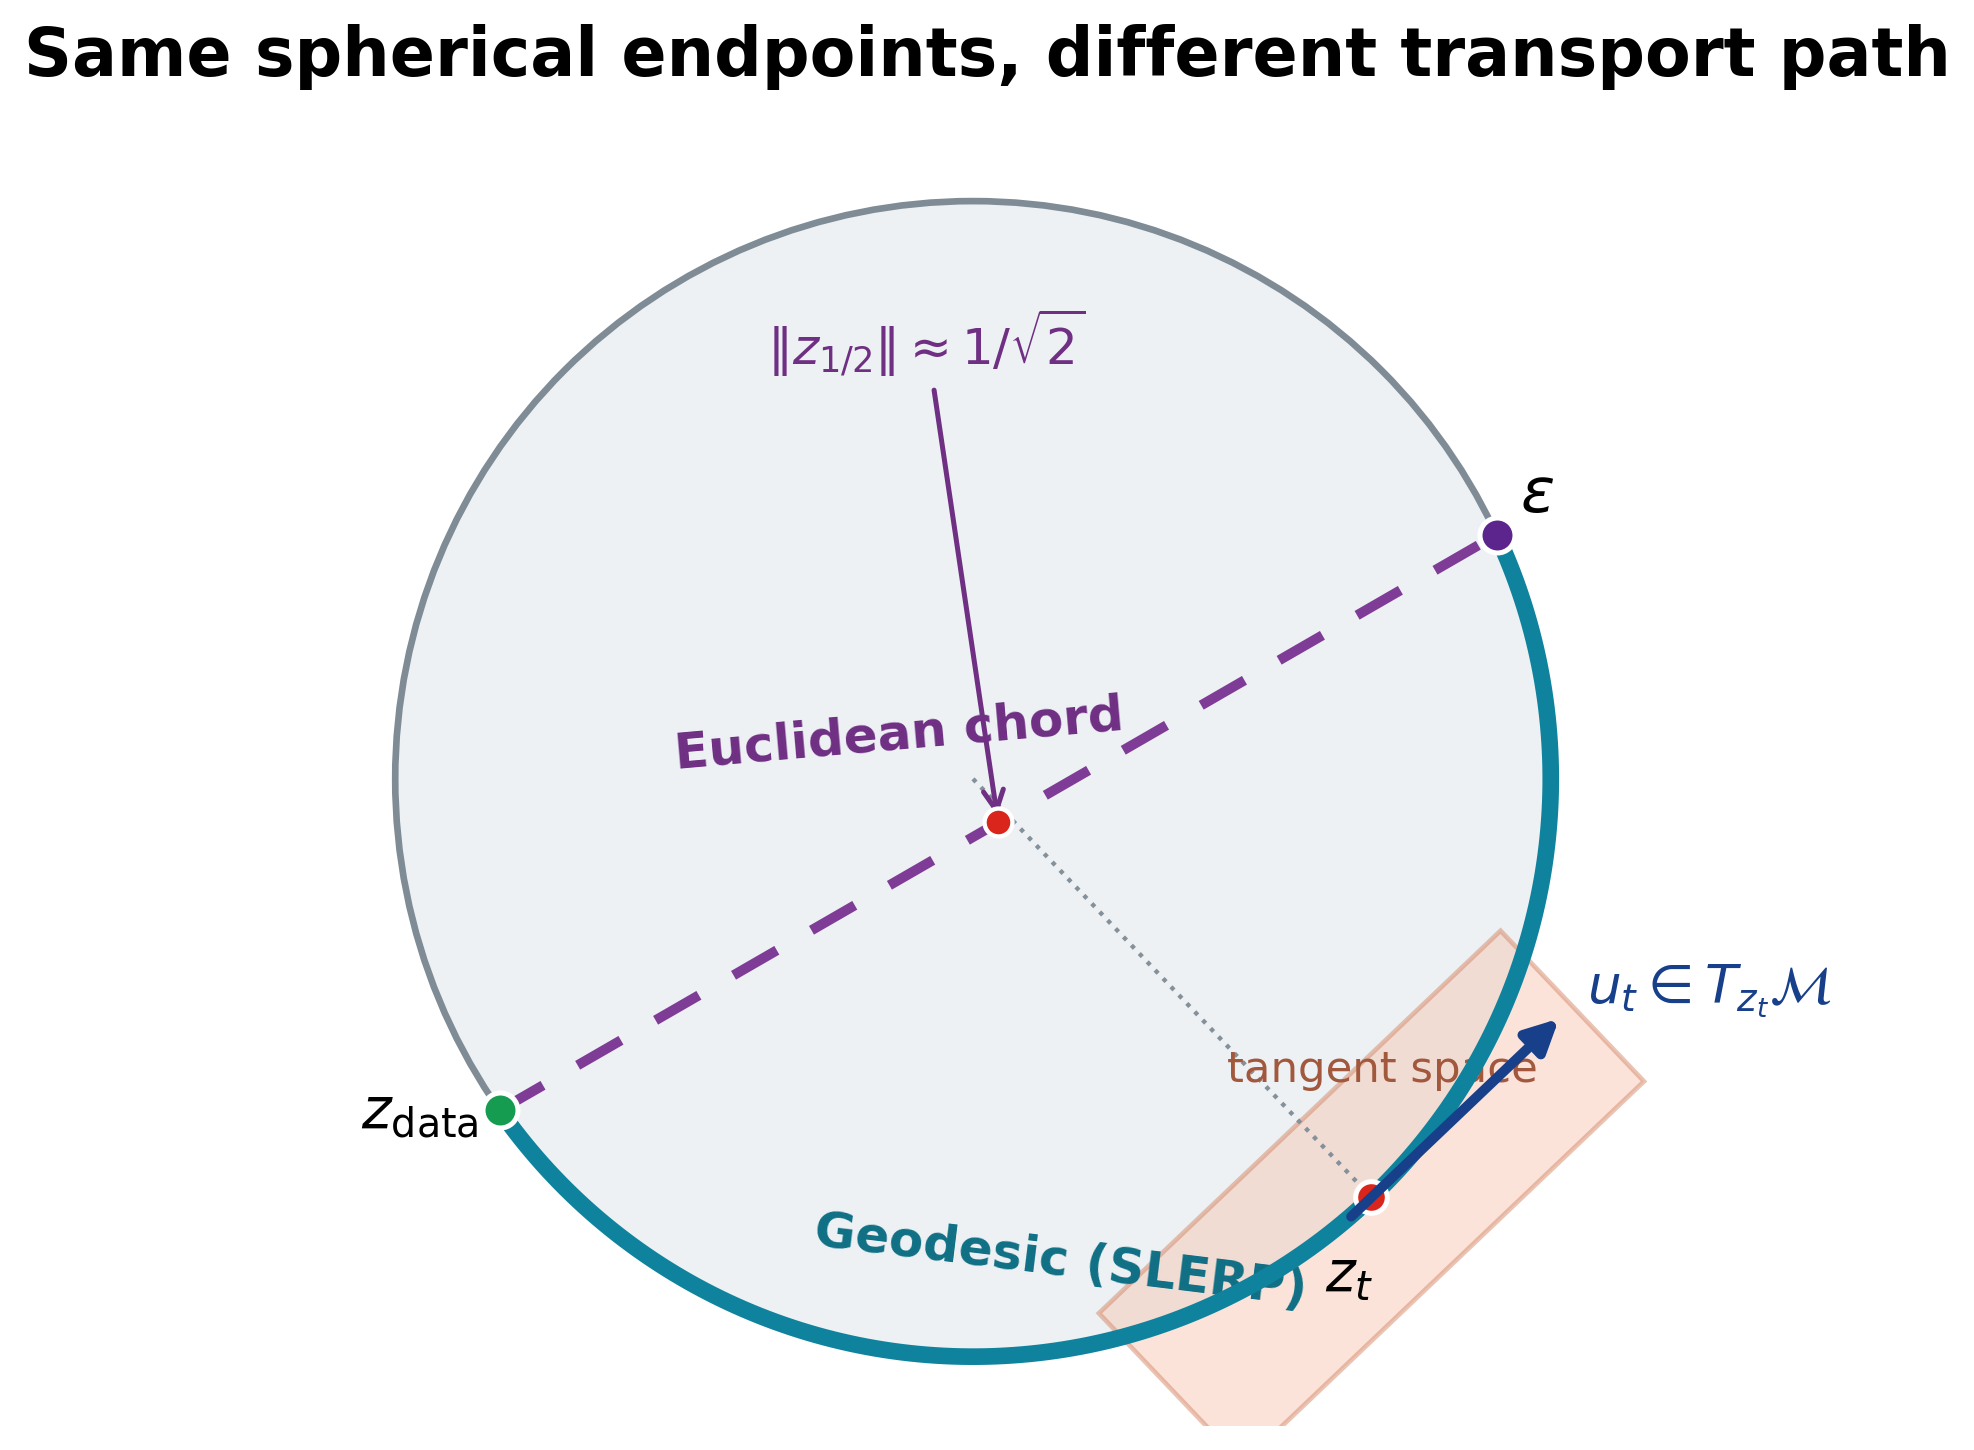
\includegraphics[width=0.55\linewidth]{assets/geometry_schematic_v9_clean.png}
\caption{With the same spherical encoder, the chord visits interior states while SRUL follows the geodesic and keeps its velocity in the tangent space.}
\label{fig:geometry}
\end{figure}

\begin{table}[H]
\centering
\small
\caption{CIFAR-10 path comparison with the same spherical autoencoder.}
\label{tab:geometry}
\setlength{\tabcolsep}{8pt}
\begin{tabular}{lrrrrr}
\toprule
Method & FID$\downarrow$ & KID$\downarrow$ & Precision$\uparrow$ & Recall$\uparrow$ & Min. norm$\uparrow$ \\
\midrule
Chord baseline & 67.44 & 0.0740 & 0.840 & 0.085 & 0.705 \\
\textbf{SRUL} & \textbf{63.84} & \textbf{0.0667} & \textbf{0.857} & \textbf{0.091} & \textbf{1.000} \\
\bottomrule
\end{tabular}
\end{table}
The geodesic improves all four image metrics and removes the radial excursion. This isolates the benefit of matching the transport path to an already-spherical representation.

\paragraph{Support matching with the same VAE.}
A VAE is a practical Euclidean latent model because KL regularization encourages a Gaussian-like latent, while its decoder still receives the complete latent vector. We keep one trained VAE encoder and decoder unchanged and vary only the prior. Standard FM models the full token $z$. Projected RFM keeps only its direction $u=z/\|z\|_2$ and restores a class/token mean radius before decoding. SRUL is shown in the same conditional evaluation because it learns spherical support before training its RFM prior.

\begin{table}[H]
\centering
\small
\caption{CIFAR-10 support-matching comparison (CFG $s=2$).}
\label{tab:support}
\setlength{\tabcolsep}{6pt}
\begin{tabular}{p{2.75cm}p{4.2cm}rrr}
\toprule
Method & Latent support and prior & FID$\downarrow$ & Precision$\uparrow$ & Recall$\uparrow$ \\
\midrule
\textbf{SRUL} & Spherical autoencoder + RFM & \textbf{49.42} & \textbf{0.857} & \textbf{0.110} \\
VAE + standard FM & Full VAE latent + linear FM & 50.70 & 0.855 & 0.091 \\
VAE + projected RFM & Directions + class/token mean radius & 56.04 & 0.848 & 0.063 \\
\bottomrule
\end{tabular}
\end{table}

The VAE token radii have coefficient of variation $0.291$, so magnitude is not constant. Replacing sample-specific radii with class/token means raises reconstruction FID from $16.90$ to $22.46$; forcing unit radius gives $113.00$. Standard FM preserves the full VAE latent and reaches FID $50.70$. Projected RFM removes sample-specific radius information and worsens FID to $56.04$. SRUL learns spherical support before RFM and reaches FID $49.42$. The result shows that the autoencoder and prior should be trained for the same support.

\subsection*{Control ablations}
We train a separate conditional SRUL prior for each tangent-noise value. Increasing $\sigma_{\mathrm{enc}}$ removes more image information and worsens both reconstruction and generation; $0.05$ is the best tested value. We then vary CFG while leaving the representation and RFM objective unchanged. Stronger guidance improves FID and precision, but reduces recall.

\begin{table}[H]
\centering
\scriptsize
\caption{CIFAR-10 tangent-noise and classifier-free-guidance ablations.}
\label{tab:controls}
\setlength{\tabcolsep}{4.1pt}
\begin{tabular}{crrr|crrr}
\toprule
$\sigma_{\mathrm{enc}}$ & Recon. FID$\downarrow$ & Gen. FID$\downarrow$ & Recall$\uparrow$ & CFG $s$ & FID$\downarrow$ & Precision$\uparrow$ & Recall$\uparrow$ \\
\midrule
0.05 & \textbf{17.53} & \textbf{48.71} & 0.090 & 1.0 & 62.44 & 0.854 & \textbf{0.083} \\
0.15 & 19.56 & 51.61 & \textbf{0.090} & 1.5 & 54.83 & 0.865 & 0.071 \\
0.30 & 27.85 & 58.16 & 0.073 & 2.0 & \textbf{49.39} & \textbf{0.884} & 0.059 \\
\bottomrule
\end{tabular}
\end{table}

\subsection*{Evaluation across image domains}
The same spatial spherical representation and RFM prior are evaluated in three settings. CIFAR-10 provides controlled geometry and sampling tests, PathMNIST evaluates texture-dominated histopathology, and CelebA-64 tests a larger token grid on structured facial images.

\begin{table}[H]
\centering
\scriptsize
\caption{Selected SRUL results. Each row is evaluated against the real split of that dataset.}
\label{tab:domains}
\setlength{\tabcolsep}{2.8pt}
\renewcommand{\arraystretch}{1.08}
\begin{tabular}{p{1.25cm}p{3.0cm}p{2.2cm}rrrr}
\toprule
Dataset & Evaluation setting & Grid / selected controls & Recon. FID & Gen. FID & Precision & Recall \\
\midrule
CIFAR-10 & Natural-object geometry and sampling study & $4\times4$; $\sigma_{\mathrm{enc}}=0.05$, $s=2$ & 17.53 & 48.71 & 0.861 & 0.090 \\
PathMNIST & Histopathology texture transfer & $4\times4$; $\sigma_{\mathrm{enc}}=0.15$, $s=2$ & 7.13 & 29.36 & 0.829 & 0.309 \\
CelebA-64 & $64\times64$ facial-image scale-up & $8\times8$; $\sigma_{\mathrm{enc}}=0.15$, $s=2$ & 9.08 & 41.22 & 0.657 & 0.198 \\
\bottomrule
\end{tabular}
\end{table}
The same design transfers to PathMNIST tissue texture and scales to an $8\times8$ grid for CelebA-64 faces.

\section{Conclusion}
SRUL trains spatial unit-norm tokens and an RFM prior on the same product-of-spheres support. With the spherical autoencoder unchanged, geodesic transport improves FID from $67.44$ to $63.84$ over a straight chord. With the same trained VAE, standard FM on the full latent reaches $50.70$, while post-hoc projection to directions before RFM worsens FID to $56.04$. These results support a simple conclusion: the autoencoder should learn the support that its prior is designed to model.

\clearpage
{\small
\begin{thebibliography}{10}
\bibitem{vae} D. P. Kingma and M. Welling. Auto-Encoding Variational Bayes. ICLR, 2014.
\bibitem{ldm} R. Rombach, A. Blattmann, D. Lorenz, P. Esser, and B. Ommer. High-resolution image synthesis with latent diffusion models. CVPR, 2022.
\bibitem{fm} Y. Lipman, R. T. Q. Chen, H. Ben-Hamu, M. Nickel, and M. Le. Flow matching for generative modeling. ICLR, 2023.
\bibitem{rjf} A. Kumar and V. M. Patel. Learning on the Manifold: Unlocking Standard Diffusion Transformers with Representation Encoders. arXiv, 2026.
\bibitem{sphere} Z. Yue et al. Image Generation with a Sphere Encoder. arXiv, 2026.
\bibitem{ul} J. Heek et al. Unified Latents: Controlling Information Flow in Latent Generative Models. arXiv, 2026.
\bibitem{cifar} A. Krizhevsky. Learning Multiple Layers of Features from Tiny Images. Technical report, 2009.
\bibitem{medmnist} J. Yang, R. Shi, D. Wei, et al. MedMNIST v2: A Large-Scale Lightweight Benchmark for 2D and 3D Biomedical Image Classification. Scientific Data, 2023.
\bibitem{celeba} Z. Liu, P. Luo, X. Wang, and X. Tang. Deep Learning Face Attributes in the Wild. ICCV, 2015.
\end{thebibliography}}
\end{document}
